%----------------------------------------------------------------------------------------
%	PACKAGES AND OTHER DOCUMENT CONFIGURATIONS
%----------------------------------------------------------------------------------------
\documentclass[12pt]{article}
\usepackage{graphicx}
\usepackage{amsmath,amsfonts,stmaryrd,amssymb} % Math packages
\usepackage{bm}
\usepackage{steinmetz}
\usepackage{enumitem}
\graphicspath{{images/}}
\usepackage{float}
\usepackage{bytefield}
\usepackage{hyperref}
\usepackage[figuresright]{rotating}
\hypersetup{
	colorlinks=true,
	linkcolor=blue,
	filecolor=magenta,      
	urlcolor=cyan,
	pdftitle={Overleaf Example},
	pdfpagemode=FullScreen,
}
\urlstyle{same}
\usepackage{mathtools}
\usepackage{fancyhdr}
\usepackage{xcolor}
\usepackage[american,RPvoltages]{circuiTikz}
\usepackage{tikz, tikz-cd}
\usepackage{pgfplots}
\usepackage{siunitx}
\usetikzlibrary{spy,shapes,arrows, arrows.meta, bending, decorations.markings}
\pgfplotsset{width=10cm,compat=1.18}
\usepackage{lmodern} % package for changing font size
\usepackage{lastpage}
\renewcommand{\figurename}{Figura}
\usepackage{tcolorbox}
\usepackage{lipsum}
%\usepackage{enumerate} % Custom item numbers for enumerations
\usepackage[ruled]{algorithm2e} % Algorithms
\usepackage[framemethod=tikz]{mdframed} % Allows defining custom boxed/framed environments
\usepackage{listings} % File listings, with syntax highlighting
%\lstset{basicstyle=\ttfamily,} % Typeset listings in monospace font
\usepackage{lipsum}
\tcbuselibrary{listings,theorems,skins,vignette,raster,breakable,magazine,poster,fitting,hooks}
\usepackage[T1]{fontenc}
\usepackage{tgbonum}
 \fontfamily{garamond}
\definecolor{myblue}{RGB}{24, 51, 73}
\definecolor{codegreen}{rgb}{0,0.6,0}
\definecolor{codegray}{rgb}{0.5,0.5,0.5}
\definecolor{codepurple}{rgb}{0.58,0,0.82}
\definecolor{backcolour}{rgb}{0.95,0.95,0.92}
\definecolor{keywords_color}{RGB}{76,146,189}
\definecolor{string_color}{RGB}{119,44,48}

\lstset{emph={%  
		"Logging":, LogLevel%
	},emphstyle={\color{yellow}\bfseries\underbar}%
}%


\lstdefinestyle{mystyle}{
	otherkeywords = {Logging,LogLevel,Default,Microsoft,Microsoft.Hosting.Lifetime,PublicKey,client_id,ConnectionStrings,Default,JabilCore,AssemblyJabilCoreRepository,Services,Context,DBType,InjectionType,IsEncrypted,UseMigration,ProjectMigration,ConnectionStringName,ServiceAssemblyPath,RepositoryAssemblyPath,JabilLogging,Host,UserName,Password,Port},
	backgroundcolor=\color{backcolour},   
	commentstyle=\color{codegreen},
	keywordstyle=\color{blue},
	numberstyle=\tiny\color{codegray},
	stringstyle=\color{red},
	basicstyle=\ttfamily\footnotesize,
	breakatwhitespace=false,         
	breaklines=true,                 
	captionpos=b,                    
	keepspaces=true,                 
	numbers=left,
	fontadjust=true,                    
	numbersep=5pt,                  
	showspaces=false,                
	showstringspaces=false,
	showtabs=false,                  
	tabsize=2
}

\lstset{style=mystyle}
%----------------------------------------------------------------------------------------
%	DOCUMENT MARGINS
%----------------------------------------------------------------------------------------

\usepackage{geometry} % Required for adjusting page dimensions and margins
\geometry{
	paper=a4paper, % Paper size, change to letterpaper for US letter size
	top=2.5cm, % Top margin
	bottom=3cm, % Bottom margin
	left=2cm, % Left margin
	right=2.5cm, % Right margin
	headheight=14pt, % Header height
	footskip=1.5cm, % Space from the bottom margin to the baseline of the footer
	headsep=1.2cm, % Space from the top margin to the baseline of the header
	%showframe, % Uncomment to show how the type block is set on the page
}

%----------------------------------------------------------------------------------------
%	FONTS
%----------------------------------------------------------------------------------------

\usepackage[utf8]{inputenc} % Required for inputting international characters
\usepackage[T1]{fontenc} % Output font encoding for international characters
\usepackage{XCharter} % Use the XCharter fonts
\usepackage{tgbonum}

\makeatletter
\pgfcircdeclarebipole{}{\ctikzvalof{bipoles/vsourcesin/height}}{sVpm}{\ctikzvalof{bipoles/vsourcesin/height}}{\ctikzvalof{bipoles/vsourcesin/width}}{
	
	\pgfsetlinewidth{\pgfkeysvalueof{/tikz/circuitikz/bipoles/thickness}\pgfstartlinewidth}
	\pgfpathellipse{\pgfpointorigin}{\pgfpoint{0}{\pgf@circ@res@up}}{\pgfpoint{\pgf@circ@res@left}{0}}
	\pgfusepath{draw}     
	\pgftext[bottom,rotate=90,y=\ctikzvalof{bipoles/vsourceam/margin}\pgf@circ@res@down]{\scriptsize$-$}
	\pgftext[top,rotate=90,y=\ctikzvalof{bipoles/vsourceam/margin}\pgf@circ@res@up]{\scriptsize$+$}
	
	\pgf@circ@res@up = .35\pgf@circ@res@up
	\pgfscope
	\pgftransformrotate{90}
	\pgfpathmoveto{\pgfpoint{-\pgf@circ@res@up}{0cm}}
	\pgfpathsine{\pgfpoint{.5\pgf@circ@res@up}{.4\pgf@circ@res@up}}
	\pgfpathcosine{\pgfpoint{.5\pgf@circ@res@up}{-.4\pgf@circ@res@up}}
	\pgfpathsine{\pgfpoint{.5\pgf@circ@res@up}{-.4\pgf@circ@res@up}}
	\pgfpathcosine{\pgfpoint{.5\pgf@circ@res@up}{.4\pgf@circ@res@up}}
	\pgfusepath{draw}
	\endpgfscope
}
\def\pgf@circ@sVpm@path#1{\pgf@circ@bipole@path{sVpm}{#1}}
\compattikzset{sinusoidal voltage source pm/.style = {\circuitikzbasekey, /tikz/to path=\pgf@circ@sVpm@path, \circuitikzbasekey/bipole/is voltage=true, \circuitikzbasekey/bipole/is voltageoutsideofsymbol=true, v=#1 }}
\compattikzset{sVpm/.style = {\comnpatname sinusoidal voltage source pm = #1}}

\pgfcircdeclarebipole{}{\ctikzvalof{bipoles/vsourcesin/height}}{sVpmh}{\ctikzvalof{bipoles/vsourcesin/height}}{\ctikzvalof{bipoles/vsourcesin/width}}{
	
	\pgfsetlinewidth{\pgfkeysvalueof{/tikz/circuitikz/bipoles/thickness}\pgfstartlinewidth}
	\pgfpathellipse{\pgfpointorigin}{\pgfpoint{0}{\pgf@circ@res@up}}{\pgfpoint{\pgf@circ@res@left}{0}}
	\pgfusepath{draw}     
	\pgftext[center,x=0.2\pgf@circ@res@down-\ctikzvalof{bipoles/vsourceam/margin}\pgf@circ@res@down]{\scriptsize$-$}
	\pgftext[top,rotate=90,y=\ctikzvalof{bipoles/vsourceam/margin}\pgf@circ@res@up]{\scriptsize$+$}
	
	\pgf@circ@res@up = .35\pgf@circ@res@up
	\pgfscope
	\pgftransformrotate{90}
	\pgfpathmoveto{\pgfpoint{-\pgf@circ@res@up}{0cm}}
	\pgfpathsine{\pgfpoint{.5\pgf@circ@res@up}{.4\pgf@circ@res@up}}
	\pgfpathcosine{\pgfpoint{.5\pgf@circ@res@up}{-.4\pgf@circ@res@up}}
	\pgfpathsine{\pgfpoint{.5\pgf@circ@res@up}{-.4\pgf@circ@res@up}}
	\pgfpathcosine{\pgfpoint{.5\pgf@circ@res@up}{.4\pgf@circ@res@up}}
	\pgfusepath{draw}
	\endpgfscope
}
\def\pgf@circ@sVpmh@path#1{\pgf@circ@bipole@path{sVpmh}{#1}}
\compattikzset{sinusoidal voltage source pmh/.style = {\circuitikzbasekey, /tikz/to path=\pgf@circ@sVpmh@path, \circuitikzbasekey/bipole/is voltage=true, \circuitikzbasekey/bipole/is voltageoutsideofsymbol=true, v=#1 }}
\compattikzset{sVpmh/.style = {\comnpatname sinusoidal voltage source pmh = #1}}
\makeatother


%----------------------------------------------------------------------------------------
%	BEGIN DOCUMENT
%----------------------------------------------------------------------------------------

\begin{document}
	%\thispagestyle{empty}
	\begin{tikzpicture}[remember picture, overlay]
		\node[anchor=north west, inner sep=0pt] at (current page.north west) {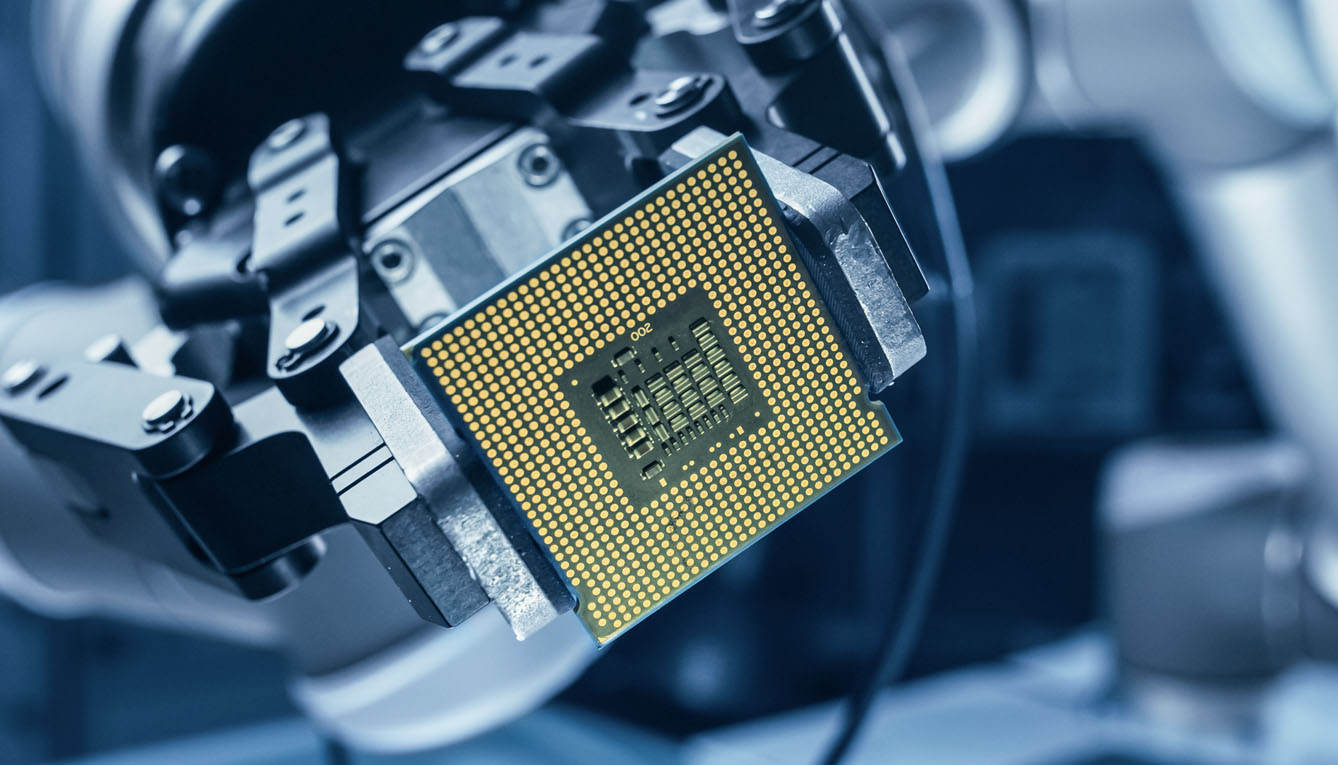
\includegraphics[width=\paperwidth, height=.5\paperheight]{picture1}};
	\end{tikzpicture}

	\vspace{13cm}
	\noindent \textcolor{myblue}{\fontsize{40pt}{40pt}\selectfont \textbf{Fuente de corriente Widlar}}\\\\\\
	{\fontsize{18pt}{18pt}\selectfont 12 de Agosto del 2023} 
	
	\newpage
	\section*{Bitwise AND}
	\subsection*{Verificando el estado de un bit}
	Un uso común de la operación \texttt{AND} bit a bit es verificar si un bit en particular en el operando se encuentra en estado \texttt{ON} u \texttt{OFF}. Por ejemplo sea el siguiente patrón de bits del cual queremos determinar si el cuarto bit se encuentra en \texttt{ON} o en \texttt{OFF}.	\\
	
	\newcommand{\bitlabel}[2]{%
		\bitbox[]{#1}{%
			\raisebox{0pt}[4ex][0pt]{%
				\turnbox{}{\fontsize{7}{7}\selectfont#2}%
			}%
		}%
	}
		\begin{center}
			\begin{bytefield}[endianness=big,bitwidth=2em]{8}
				\bitheader[lsb=1]{1-8} \\
				\bitbox{1}{1} & \bitbox{1}{0} & \bitbox{1}{1} & \bitbox{1}{0} & \bitbox{1}{1} & \bitbox{1}{1} & \bitbox{1}{0} & \bitbox{1}{1}  
			\end{bytefield}	
		\end{center}
	
	\noindent Ya que queremos determinar el estado del cuarto bit, utilizaremos un segundo operando con el siguiente contenido el cual representa el número 8 en decimal. Esta secuencia de bits es llamada \textbf{Bit Mask}.
	\begin{center}
		\begin{bytefield}[endianness=big,bitwidth=2em]{8}
			\bitlabel{1}{$2^7$} & \bitlabel{1}{$2^6$} \bitlabel{1}{$2^5$} & \bitlabel{1}{$2^4$} & \bitlabel{1}{$2^3$} & \bitlabel{1}{$2^2$} & \bitlabel{1}{$2^1$} & \bitlabel{1}{$2^0$} \\
			\bitheader[lsb=1]{1-8} \\
			\bitbox{1}{0} & \bitbox{1}{0} & \bitbox{1}{0} & \bitbox{1}{0} & \bitbox{1}{1} & \bitbox{1}{0} & \bitbox{1}{0} & \bitbox{1}{0}  
		\end{bytefield}	
	\end{center}
	
	\noindent El resultado de realizar la operación \texttt{AND} a los bits de la misma posición en el primer y segundo operando obtenemos:
\begin{center}
	\begin{bytefield}[endianness=big,bitwidth=2em]{8}
		\bitheader[lsb=1]{1-8} \\
		\bitbox{1}{1} & \bitbox{1}{0} & \bitbox{1}{0} & \bitbox{1}{0} & \bitbox{1}{1} & \bitbox{1}{0} & \bitbox{1}{0} & \bitbox{1}{0}  
	\end{bytefield}	
\end{center}
	
\noindent El siguiente programa muestra un código de ejemplo para determinar el estado del  \texttt{n-ésimo} bit de una determinada cantidad.
	\begin{lstlisting}[language={C}]
		/*
		+----------+---+---+---+---+---+---+---+---+
		| Position | 8 | 7 | 6 | 5 | 4 | 3 | 2 | 1 |
		+----------+---+---+---+---+---+---+---+---+
		| Bits     | 1 | 0 | 1 | 0 | 1 | 1 | 0 | 1 |
		+----------+---+---+---+---+---+---+---+---+ */
		
		#include<stdio.h>
		#include<stdlib.h>
		#include<math.h>
		
		int value;
		int position;
		int posToDec;
		int bitMask;
		
		printf("%s", "Enter the quantity in decimal format: ");
		scanf("%d", &value);
		printf("%s", "Enter the bit's position you want to supervise: ");
		scanf("%d", &position);
		
		posToDec = pow(2, position - 1);
		bitMask = value & posToDec;
		
		if (bitMask == 0)
			printf("The bit position number %d is OFF", position);
		else
			printf("The bit position number %d is ON", position);
	\end{lstlisting}
	
	\subsection*{Cambiando el estado de un bit de ON a OFF}
	Una segunda aplicación de la operación \texttt{AND} bit a bit es para cambiar el estado de un determinado bit, por ejemplo, sea el siguiente patrón de bits:
	
	\begin{center}
		\begin{bytefield}[endianness=big,bitwidth=2em]{8}
			\bitheader[lsb=1]{1-8} \\
			\bitbox{1}{0} & \bitbox{1}{0} & \bitbox{1}{0} & \bitbox{1}{0} & \bitbox{1}{0} & \bitbox{1}{1} & \bitbox{1}{1} & \bitbox{1}{1}  
		\end{bytefield}	
	\end{center}
	
	\noindent Y queremos cambiar el estado del segundo bit. Para esto, necesitamos un segundo operando que haga el enmascaramiento correspondiente. Esto se logra colocando todos los bits en 1 a excepción de la posición que se requiere cambiar, es decir:
	
	\begin{center}
		\begin{bytefield}[endianness=big,bitwidth=2em]{8}
			\bitheader[lsb=1]{1-8} \\
			\bitbox{1}{1} & \bitbox{1}{1} & \bitbox{1}{1} & \bitbox{1}{1} & \bitbox{1}{1} & \bitbox{1}{1} & \bitbox{1}{0} & \bitbox{1}{1}  
		\end{bytefield}	
	\end{center}
	
	\noindent Al realizar la operación \texttt{AND} a ambos operandos obtenemos
	\begin{center}
		\begin{bytefield}[endianness=big,bitwidth=2em]{8}
			\bitheader[lsb=1]{1-8} \\
			\bitbox{1}{0} & \bitbox{1}{0} & \bitbox{1}{0} & \bitbox{1}{0} & \bitbox{1}{0} & \bitbox{1}{1} & \bitbox{1}{0} & \bitbox{1}{1}  
		\end{bytefield}	
	\end{center}

\subsection*{Extrayendo un patrón de bits}

\begin{center}
	\begin{bytefield}[endianness=big,bitwidth=2em]{16}
		\bitlabel{1}{RN3} & \bitlabel{1}{RN2} \bitlabel{1}{RN1} & \bitlabel{1}{RN0} & \bitlabel{1}{CT} & \bitlabel{1}{M1} & \bitlabel{1}{M0} & \bitlabel{1}{OVF} & \bitlabel{1}{CRF} & \bitlabel{1}{FH} & \bitlabel{1}{FL} & \bitlabel{1}{L} & \bitlabel{1}{POL} & \bitlabel{1}{ME} & \bitlabel{1}{FC1} & \bitlabel{1}{FC0}\\
		\bitheader[lsb=0]{0-15} \\
		\bitbox{1}{1} & \bitbox{1}{0} & \bitbox{1}{0} & \bitbox{1}{0} & \bitbox{1}{1} & \bitbox{1}{1} & \bitbox{1}{1} & \bitbox{1}{0} & \bitbox{1}{1} & \bitbox{1}{1} & \bitbox{1}{0} & \bitbox{1}{1} & \bitbox{1}{0} & \bitbox{1}{1} & \bitbox{1}{1} & \bitbox{1}{1}
	\end{bytefield}	
	\end{center}

\end{document}